\documentclass{article}
\usepackage[T1]{fontenc}
\setlength{\paperwidth}{16cm}
\setlength{\paperheight}{19cm}
\setlength{\textwidth}{14cm}
\setlength{\textheight}{17cm}
\setlength{\oddsidemargin}{-1.54cm}
\setlength{\topmargin}{-1.54cm}
\setlength{\headheight}{0pt}
\setlength{\headsep}{0pt}
\special{papersize=16cm,19cm}
\usepackage{newtxtext}
\usepackage{amsmath}
\usepackage[varvw]{newtxmath}
\usepackage{pgfplots}
\pgfplotsset{compat=1.17}
\pagestyle{empty}
\begin{document}
\centering
\begin{tikzpicture}
\begin{axis}[
width=\linewidth,height=5.9cm,
title={x64: 13 previously low-working-rate payloads},title style={font=\small\bfseries},
ylabel={Working rate (\%)},ymin=-3,ymax=107,ytick={0,25,50,75,100},
xmin=-0.6,xmax=14.6,xtick={0,...,14},xticklabels={NOP,EQ,PII,BCF,IBP,EQ+NOP+PII,EQ+NOP+BCF,EQ+NOP+IBP,NOP+EQ,NOP+PII,NOP+BCF,NOP+IBP,EQ+PII,EQ+BCF,EQ+IBP},
xticklabel style={rotate=60,anchor=east,font=\scriptsize},
tick label style={font=\scriptsize},label style={font=\small},
ymajorgrids=true,grid style={gray!20},axis line style={gray!60},
legend style={font=\scriptsize,at={(0.98,0.98)},anchor=north east,legend columns=2,fill=white,draw=gray!25},
]
\addplot[gray!40,thick,no marks,forget plot] coordinates {(0,0.000000) (0,77.692308)};
\addplot[gray!40,thick,no marks,forget plot] coordinates {(1,0.000000) (1,100.000000)};
\addplot[gray!40,thick,no marks,forget plot] coordinates {(2,0.000000) (2,84.615385)};
\addplot[gray!40,thick,no marks,forget plot] coordinates {(3,0.000000) (3,83.846154)};
\addplot[gray!40,thick,no marks,forget plot] coordinates {(4,0.000000) (4,83.076923)};
\addplot[gray!40,thick,no marks,forget plot] coordinates {(5,0.769231) (5,65.384615)};
\addplot[gray!40,thick,no marks,forget plot] coordinates {(6,0.000000) (6,83.076923)};
\addplot[gray!40,thick,no marks,forget plot] coordinates {(7,0.000000) (7,74.615385)};
\addplot[gray!40,thick,no marks,forget plot] coordinates {(8,6.250000) (8,78.461538)};
\addplot[gray!40,thick,no marks,forget plot] coordinates {(9,0.781250) (9,66.923077)};
\addplot[gray!40,thick,no marks,forget plot] coordinates {(10,0.000000) (10,83.076923)};
\addplot[gray!40,thick,no marks,forget plot] coordinates {(11,1.550388) (11,70.769231)};
\addplot[gray!40,thick,no marks,forget plot] coordinates {(12,0.000000) (12,84.615385)};
\addplot[gray!40,thick,no marks,forget plot] coordinates {(13,7.031250) (13,83.076923)};
\addplot[gray!40,thick,no marks,forget plot] coordinates {(14,1.550388) (14,83.846154)};
\addplot[only marks,mark=o,mark size=2.2pt,gray!85] coordinates {(0,0.000000) (1,0.000000) (2,0.000000) (3,0.000000) (4,0.000000) (5,0.769231) (6,0.000000) (7,0.000000) (8,6.250000) (9,0.781250) (10,0.000000) (11,1.550388) (12,0.000000) (13,7.031250) (14,1.550388)};
\addlegendentry{Historical}
\addplot[only marks,mark=*,mark size=2.2pt,blue!65!black] coordinates {(0,77.692308) (1,100.000000) (2,84.615385) (3,83.846154) (4,83.076923) (5,65.384615) (6,83.076923) (7,74.615385) (8,78.461538) (9,66.923077) (10,83.076923) (11,70.769231) (12,84.615385) (13,83.076923) (14,83.846154)};
\addlegendentry{Updated}
\end{axis}\end{tikzpicture}
\par\vspace{0.5cm}
\begin{tikzpicture}
\begin{axis}[
width=\linewidth,height=5.9cm,
title={x86: 36 previously low-working-rate payloads},title style={font=\small\bfseries},
ylabel={Working rate (\%)},ymin=-3,ymax=107,ytick={0,25,50,75,100},
xmin=-0.6,xmax=14.6,xtick={0,...,14},xticklabels={NOP,EQ,PII,BCF,IBP,EQ+NOP+PII,EQ+NOP+BCF,EQ+NOP+IBP,NOP+EQ,NOP+PII,NOP+BCF,NOP+IBP,EQ+PII,EQ+BCF,EQ+IBP},
xticklabel style={rotate=60,anchor=east,font=\scriptsize},
tick label style={font=\scriptsize},label style={font=\small},
ymajorgrids=true,grid style={gray!20},axis line style={gray!60},
legend style={font=\scriptsize,at={(0.98,0.98)},anchor=north east,legend columns=2,fill=white,draw=gray!25},
]
\addplot[gray!40,thick,no marks,forget plot] coordinates {(0,20.833333) (0,22.222222)};
\addplot[gray!40,thick,no marks,forget plot] coordinates {(1,60.000000) (1,57.777778)};
\addplot[gray!40,thick,no marks,forget plot] coordinates {(2,0.000000) (2,25.000000)};
\addplot[gray!40,thick,no marks,forget plot] coordinates {(3,18.333333) (3,42.222222)};
\addplot[gray!40,thick,no marks,forget plot] coordinates {(4,14.166667) (4,23.888889)};
\addplot[gray!40,thick,no marks,forget plot] coordinates {(5,0.000000) (5,5.000000)};
\addplot[gray!40,thick,no marks,forget plot] coordinates {(6,11.944444) (6,31.111111)};
\addplot[gray!40,thick,no marks,forget plot] coordinates {(7,7.500000) (7,11.111111)};
\addplot[gray!40,thick,no marks,forget plot] coordinates {(8,20.277778) (8,22.222222)};
\addplot[gray!40,thick,no marks,forget plot] coordinates {(9,0.000000) (9,5.000000)};
\addplot[gray!40,thick,no marks,forget plot] coordinates {(10,17.222222) (10,30.555556)};
\addplot[gray!40,thick,no marks,forget plot] coordinates {(11,9.722222) (11,17.222222)};
\addplot[gray!40,thick,no marks,forget plot] coordinates {(12,0.000000) (12,25.000000)};
\addplot[gray!40,thick,no marks,forget plot] coordinates {(13,22.222222) (13,43.888889)};
\addplot[gray!40,thick,no marks,forget plot] coordinates {(14,12.222222) (14,26.111111)};
\addplot[only marks,mark=o,mark size=2.2pt,gray!85] coordinates {(0,20.833333) (1,60.000000) (2,0.000000) (3,18.333333) (4,14.166667) (5,0.000000) (6,11.944444) (7,7.500000) (8,20.277778) (9,0.000000) (10,17.222222) (11,9.722222) (12,0.000000) (13,22.222222) (14,12.222222)};
\addlegendentry{Historical}
\addplot[only marks,mark=*,mark size=2.2pt,blue!65!black] coordinates {(0,22.222222) (1,57.777778) (2,25.000000) (3,42.222222) (4,23.888889) (5,5.000000) (6,31.111111) (7,11.111111) (8,22.222222) (9,5.000000) (10,30.555556) (11,17.222222) (12,25.000000) (13,43.888889) (14,26.111111)};
\addlegendentry{Updated}
\end{axis}\end{tikzpicture}

\par\smallskip\small
Same 49 selected payloads, before and after the pipeline update.\\
x64: 1.2\% to 80.2\%; x86: 14.9\% to 25.9\% (pooled rates).\\
Historical and updated test counts differ; see manuscript for the protocol.
\end{document}
